\documentclass[journal]{IEEEtran}
% *** graph PACKAGES ***
%
\ifCLASSOPTIONcompsoc 
  \usepackage[caption=false,font=normalsize,labelfont=sf,textfont=sf]{subfig}
\else
  \usepackage[caption=false,font=footnotesize]{subfi g}
\fi
\usepackage{graphicx}

% *** citation PACKAGES ***
%
\ifCLASSOPTIONcompsoc
  % The IEEE Computer Society needs nocompress option
  % requires cite.sty v4.0 or later (November 2003)
  \usepackage[nocompress]{cite}
\else
  % normal IEEE
  \usepackage{cite}
\fi

% *** math PACKAGES ***
%
\usepackage{amsmath}
\usepackage{graphicx}
\usepackage{algorithmic}
\usepackage{algorithm}
\renewcommand{\algorithmicrequire}{\textbf{Input:}} 
\renewcommand{\algorithmicensure}{\textbf{Output:}}
\usepackage{amsfonts,amssymb}

% *** special symbol PACKAGES ***
%
\usepackage{tikz}
\newcommand\encircle[1]{%
  \tikz[baseline=(X.base)] 
    \node (X) [draw, shape=circle, inner sep=-1.5] {\strut #1};}

% *** table PACKAGES ***
%
% \usepackage{subtable}


\hyphenation{op-tical net-works semi-conduc-tor}



\begin{document}

\title{Reliability-aware and Deadline-constrained Mobile Service Composition over Opportunistic Networks}

\author{Qinglan Peng,
        Mengchu Zhou, ~\IEEEmembership{Fellow,~IEEE,}
        Yunni Xia, ~\IEEEmembership{Senior member,~IEEE,}
        Shuiguang Deng, ~\IEEEmembership{Senior member,~IEEE,}
        Xin Luo, ~\IEEEmembership{Senior member,~IEEE,}
        Qingsheng Zhu,
        Wanbo Zheng


\thanks{This work is in part supported by NSFC under Grant No. 61472051; Fundamental Research Funds for the Central Universities under project Nos. 106112014CDJZR185503 and CDJZR12180012; Science foundation of
Chongqing Nos. cstc2014jcyjA40010 and cstc2014jcyjA90027; Chongqing Social Undertakings and Livelihood Security Science and Technology Innovation Project Special Program No. cstc2016shmszx90002; China Postdoctoral Science Foundation No. 2015M570770; Chongqing Postdoctoral Science special Foundation No. Xm2015078; Universities’ Sci-tech Achievements Transformation Project of Chongqing No. KJZH17104.}

\thanks{Qinglan Peng, Yunni Xia, and Qingsheng Zhu are with the school of computers, Chongqing University, Chongqing 400030, China (emails: qlp@cqu.edu.cn, xiayunni@hotmail.com, qszhu@cqu.edu.cn, wbzheng2008@cqu.edu.cn)}

\thanks{X. Luo is with Chinese Academy of Sciences, Chongqing Institute of Green and Intelligent
Technology, Chongqing 400714, China (luoxin21@gmail.com)}

\thanks{M. C. Zhou is with Department of Electrical and Computer Engineering, New Jersey Institute of Technology, Newark, NJ 07102, USA (email:zhou@njit.edu).}

\thanks{Yunni Xia is the corresponding author of this work.}
}


% The paper headers
% \markboth{Journal of \LaTeX\ Class Files,~Vol.~14, No.~8, August~2015}%
% {Shell \MakeLowercase{\textit{et al.}}: Bare Demo of IEEEtran.cls for IEEE Journals}


% make the title area
\maketitle

% As a general rule, do not put math, special symbols or citations
% in the abstract or keywords.
\begin{abstract}
An opportunistic link between two mobile devices or nodes can be constructed when they are within each other's communication. Typically, cyber-physical environments consist of a number of mobile devices that are potentially able to establish opportunistic contacts and serve mobile applications in a cost-effective way.
Opportunistic mobile service computing is a promising paradigm capable of utilizing the pervasive mobile computational resources around users. Mobile users are thus allowed to exploit nearby mobile services to boost their computing power without investment into their own resource pool. 
Nevertheless, various challenges, especially its quality-of-service (QoS) and reliability-aware scheduling, are yet to be addressed. Existing studies and related scheduling strategies consider mobile users to be fully stable and available.
In this paper, instead, we propose a framework, named a mobile service opportunistic network, and a reliability-aware and deadline-constrained scheduling algorithm for service composition. 
We then formulate the problem into an optimization problem and utilize an improved Krill-Herd algorithm to solve it.
Finally, we carry out a case study based on some well-known mobile service composition templates and a real-world dataset. The comparison suggest that our proposed approach outperforms traditional approaches, especially those considering stable and fully available mobile services in their models and algorithms.
\end{abstract}

% Note that keywords are not normally used for peerreview papers.
\begin{IEEEkeywords}
Mobile Computing, Mobile Opportunistic Network, Mobile Service Composition, Service Reliability.
\end{IEEEkeywords}

~\\
\noindent List of abbreviations:
~\\

\noindent
\begin{tabular}{@{} l p{7.36cm} }
\textbf{C2M}   &   Cloud to Mobile pattern\\
\textbf{DE}    &   Differential Evolution \\
\textbf{D2D}   &   Device to Device communications \\
\textbf{GA}    &   Genetic Algorithm \\
\textbf{KH}    &   Krill-Herd algorithm \\
\textbf{M2M}   &   Mobile to Mobile pattern \\
\textbf{PSO}   &   Particle Swarm Optimization \\
\end{tabular}

\noindent \textbf{RWP}   $\ $   Random way point mobility model \\
\noindent \textbf{QoS}   $\ \ \, $   Quality of Service \\
\noindent \textbf{SGA}   $\ \; $   Stud Genetic algorithm \\
\noindent \textbf{SLA}   $\ \ $   Service-level-agreement \\

\noindent List of symbols: 
~\\

\noindent
\begin{tabular}{@{} l p{7.36cm} }
$\alpha$      &   Half of service consumer central angle \\
$\beta$       &   Half of service provider central angle \\
$\gamma_{i}$  &   The estimated time that all earlier tasks scheduled to the same candidate service to $t_i$ are accomplished  \\
$\delta$      &   The time between the arrival of a service composition request and the generation of its corresponding schedule \\
$\tau$        &   The estimated complement time of a service composition \\
$A(s)$      &   The function to identify availability of mobile service $s$ \\
$b_i$         &   The estimated start time of $t_i$ \\
$C_{r}$       &   The crossover rate of a KH algorithm \\
$C_{v}$       &   The crossover vector of a KH algorithm \\
% $CT$          &   The estimated completion time of a schedule plan \\
$d_i$         &   The estimated end time of $t_i$ \\
$D$           &   The user-recommended constraint of the completion time of a service composition \\
$D_i$         &   The random physical diffusion of a krill individual \\
$D_{i,k}$     &   The data transfer time between $t_i$ and $t_k$ \\
$e_i$         &   The estimated execution time of $t_i$ \\
$e_{i,j}$     &   The edge connecting $t_i$ and $t_j$ \\
$F_i$         &   The foraging action of a krill individual \\ 
% $G$           &   The max iteration count of a KH algorithm \\
$G$           &   The number of max iteration generations of a KH algorithm \\
$N_i$         &   The motion influenced by other krills \\
$P$           &   The resources pool of available mobile services \\
$R$           &   Transmission range of a mobile device \\
$S$           &   The population size of a KH algorithm \\
$t_i$         &   The $i$-th task of a service composition \\
$\bar{t}$     &   The average service time of a concrete service \\
$t_{entry}$   &   The dummy start task of a service composition \\
$t_{exit}$    &   The dummy end task of a service composition \\
$w(t_i)$      &   The function to identify the concrete service that $t_i$ is scheduled into \\
$X$           &   The population of krills \\
$X_i$         &   The $i$-th individual in a krill population \\
$y_i$         &   The estimated earliest time that all immediately preceding tasks successfully terminate and transfer data \\
\end{tabular}
~\\

\IEEEpeerreviewmaketitle

\section{Introduction}

\IEEEPARstart{R}{ecent years} have witnessed the rapid development of mobile devices (e.g., smartphones, tablets, wearable devices, etc.) and mobile communication.
Mobile devices are changing the way people getting the information and their daily lives.
These devices allow them to enjoy multiple ways of communicating almost anywhere at anytime \cite{satyanarayanan2010mobile}.

The number of mobile devices is rapidly growing and it has already surpassed the number of stationary Internet hosts.
Mobile services are also developed and provided at a significant rate, while, the requirements from mobile users are becoming more demanding, i.e., more complicated applications are needed to be run on mobile devices such as virtual reality applications \cite{bastug2017toward} or machine learning applications \cite{abadi2016TensorFlow} on mobile phones. However, because of the limited hardware resources of mobile devices (e.g., computational resource, battery life, memory, and storage), these resource-intensive tasks are usually offloaded to mobile computing cloud \cite{dinh2013survey}, which result in high data transfer cost (energy cost and communication fee) and high latency.

Opportunistic computing is a promising complementary to conventional mobile cloud computing. As illustrated in Fig. 1, the basic idea of opportunistic computing is to allow users to utilize the resources and services that other users share, by exploiting the direct physical contacts among users, and the resulting potential to exchange data through a direct connection between their devices (e.g., through Wi-Fi or Bluetooth). Resources and services available on mobile devices can be directly shared among users in a elastic and on-demand way without time-consuming and energy-requiring interactions with pre-existing infrastructure, either at the networking level (e.g., cellular networks) or at the computing/service level (e.g., the mobile computing cloud). 
Note that, mobile tasks usually require huge computational resources or data transfer (e.g., TensorFlow on mobile, Video editor on mobile and Online video). Nearby mobile service provider are thus more adept, in terms of energy-efficiency, at executing these tasks than the online services or nodes with the help of device to device (D2D) communications such as Bluetooth, Wi-Fi and NFC \cite{balani2007energy}. D2D communications are featured with extensively-reduced data transfer delays and required energy than the traditional cellular network. Thus it provides better user-perceived service quality in terms of reduced waiting time and improved service responsiveness. It is widely believed to have potential to replenish traditional cellular communications by providing increased user throughput, reduced cellular traffic, and extened network coverage.

However, because of the completely different application patterns compared with traditional service computing, service computing in mobile environment faces two inherent challenges.

1) Unguaranteed reliability: Mobile users may change their locations very frequently in a mobile environment and thus service availability tends to be fluctuating and time-varying. It is therefore difficult to guarantee high reliability of service composition when their underlying mobile services are of time-varying availability or even unavailable. Thus, determining how to handle service availability is a major challenge for providing reliable mobile services in highly dynamic mobile environments.

2) Neglect of deadline-constrain: Different from large scientific workflows executed in stationary IaaS cloud for hours, a mobile service composition usually completed within a few seconds to tens of seconds in a highly dynamic mobile environment. Some studies, e.g., \cite{Niida2010} and \cite{zhou2016define} , have concluded that mobile users can tolerance a certain maximum time for a composition request. Once timeout happens, they may lose their patience and interrupt requested service thus result in failure. More specifically, if a service composition algorithm does not consider deadline-constrain, it is more likely to generate composition schedules with high makespan which brings bad user experience and result in high SLA (Service-level-agreement) violated rate. Thus, it is necessary to introduce deadline-constrained mechanism in such a highly dynamic mobile environments.

\begin{figure}[!t]
\centering
\includegraphics[width=3.5in]{./img/pic1.pdf}
\caption{Opportunistic computing}
\label{Opportunistic computing}
\end{figure}

% 1) Constant Mobility: Mobile users may change their locations very frequently in mobile environment and thus service availability could be fluctuating and time-varying. It is therefore difficult to guarantee high reliability of service composition when their underlying mobile services are with time-varying availability or even unavailable. Thus, determining how to handle service availability is a major challenge for providing reliable mobile services in highly dynamic mobile environments.

% 2) Limited Resource: mobile devices have limited computing capability compared with stationary ones. Designing scheduling algorithms with high time-complexity should be avoided.
%Moreover, such algorithms are supposed to be highly time-efficient because mobile services themselves are with time-varying availability/QoS and only fast ones avoid ineffective scheduling, as well. 
%Nevertheless, the underlying problem for optimal scheduling and composition is well acknowledged to be NP-hard. It is therefore a great challenge to guarantee both low time-complexity and optimality of such algorithms.

To address the aforementioned challenges and concerns in this work, we propose a reliability-aware and deadline-constrained mobile service composition approach, where mobile users in a mobile service opportunistic network are allowed to combine and exploit, through D2D communications, nearby devices' resources. Instead of assuming fully available mobile services, we consider time-varying availability of services due to their run-time mobility and develop reliability-aware deadline/reliability estimation models for service compositions. Based on the estimation model, we present a Krill-Herd-based algorithm to decide optimal composition schedules at run-time aiming at maximized reliability with guaranteed deadline. To validate our proposed approach, we carry out a case study based on some well-known mobile service composition templates and a real-world dataset (the D2D contact traces of MIT Reality dataset and the response time data of the QWS dataset).

\section{RELATED WORK}

\subsection{Mobile opportunistic network}
Opportunistic networking is one of the most promising evolutions of the traditional multi-hop one. 
Instead of relying itself on stable end-to-end paths through Internet, opportunistic networks do not consider node mobility a problem but as useful opportunity. 
Extensive efforts have been made into this direction. For example, Marco \emph{et al}. \cite{Conti2014} give a review of opportunistic networks and regard it as the first step in people-centric networking. They also discuss challenges to be addressed, especially the mobility modeling and routing-plan decision problems.
Turkes \emph{et al}. \cite{turkes2016cocoon} propose a middleware named Cocoon for a mobile opportunistic network. They design a routing protocol on Wi-Fi and Bluetooth connections and and show that their proposed protocol performs well in terms of dissemination rate, delivery latency and energy consumption.
Giordano \emph{et al}. \cite{giordano2011human} consider mobile clouds supported by opportunistic computing, where a mobile device can combine and exploit heterogeneous resources from other devices.
Pu \emph{et al}. \cite{Pu2017crowd} present a QoS-oriented self-organized mobile crowdsourcing framework where prevalent opportunistic user encounters in our daily life are utilized to solve a crowdsourcing problem.
Zhan \emph{el al}. \cite{zhan2017time} propose a time-sensitive incentive-aware mechanism for mobile opportunistic crowdsensing. They formulate the interaction between a data carrier and mobile relay users as a two-player cooperative game and apply an asymmetric Nash bargain strategy to obtain the optimal cooperation plan.

\subsection{Mobile service composition}
Mobile service composition refers to the technique of creating composite services with the help of smaller, simpler and easily executable services or components over mobile networks. Recent technological advances in novel mobile device design and development as well as wireless networking materialize a vision where devices all around a user, either embedded as a part of smart spaces, or being carried by other users
near by, are enabled to present services probably useful. Users sometimes look for services that are not pre-existent on any device. Otherwise, they dynamically build new services by appropriately combining already existing ones. Extensive studies are carried out in this direction. 
For example, Deng \emph{et al}. \cite{Deng2016} classify mobile service composition methods into three categories: Cloud to Mobile (C2M), Mobile to Mobile (M2M) and Hybrid. They also discuss related challenges, e.g., performance guarantee, energy efficiency, and security.
Later, Deng \emph{et al}. \cite{Deng2017} propose a mobile-service-sharing-community model and extend the random way point (RWP) model to model user mobility. They utilize a meta-heuristic algorithm to decide the optimal compositional plan. They consider services shared in a community are fully available all the time.
Sadiq \emph{et al}. \cite{sadiq2015service} use a Levy walk model and SLAW model to generate user traces, where each node is equally likely to meet any other one. Reachability between devices are guaranteed and supported by their multi-hop connections when their end-to-end connected paths fail.
Christin Groba \emph{et al}. \cite{groba2014opportunistic} present a novel service composition protocol that allocates and invokes service providers opportunistically to minimize the impact of topology changes. However, their protocol only support a sequences and parallel service flows.
Yang \emph{et al}. \cite{Yang2010} present a comprehensive QoS model for pervasive services. They consider not only mobile wireless network characteristics but also user-perceived factors. However, their algorithm considers single service selection rather than multiple service selection for composite service processes.
Zhang \emph{et al}. \cite{Zhang2016qos} consider a bio-inspired and context-aware mobile service selection algorithm. They introduce a tree-encoding method to improve the capacity and efficiency of genetic operations of a genetic algorithm. However, for simplicity, they do not consider user mobility.
Wang \emph{et al}. \cite{wang2011exploiting} employ a probability-free model and a probabilistic model to characterize the uncertainty during service invoking. They assume that services are able to tolerate a certain level of the mobility of service providers. However, for simplicity, they consider the sequential pattern of service compositions only.

\begin{figure}[!t]
\centering
\includegraphics[width=3.5in]{./img/pic2.pdf}
\caption{Mobile services composition over opportunistic network}
\label{fig_MSCON}
\end{figure}

It can be seen that, existing studies are limited in several ways: 
1) for simplicity, most of them consider fully-available services in their QoS determination models and scheduling algorithms. However, real-world mobile services are usually of unreliable and time-varying availability, as suggested by our test data given later.
2) Various studies consider RWP and Levy models where mobile devices are assumed to follow random walks and Brownian motion patterns. However, recent several studies, e.g., \cite{barbosa2017human, bettstetter2003node, navidi2004improving}, show that individual trajectories are far from random, possessing a high degree of regularity and predictability. Different mobility model must be applied to different application environment \cite{camp2002survey}, e.g., mobility pattern of office is different from that of subway. Thus, using a general model to describe such different mobility patterns is unrealistic.
3) Some, e.g., \cite{wang2011exploiting, Deng2016-2} use a probabilistic model to characterize the uncertainty of composite services and consider that unavailability of composing concrete services leads to failure of service compositions.
They assume the probability that a provider stays within the required distance to its corresponding service requester follows a certain type of given distribution. However, such distribution in real-world is usually unpredictable due to the uncertain spatial layout of mobile devices and the human traffic pattern (e.g., people flow in a fixed office cubicle is totally different from that of a crowded shopping mall). 

The above limitations could be well avoided by using a reliability-aware and deadline-constrained service composition mechanism and a Krill-Herd-based algorithm to decide composition schedules, where the reliability of a composition schedule which can be obtained by aggregating availability of its tasks is adopted as an optimization objective to improve success rate of mobile service composition.

\section{modeling reliability-aware mobile service composition}

\subsection{Mobile Service Composition over Opportunistic Network Framework}

Mobile service composition over an opportunistic network has three properties:

1) Locality: Rather than on stable Internet, it is based on mobile networks and exploits local user mobility. Mobile users can perceive nearby services and establish self-organized local communication within permitted transmission distance.

2) Mobility: Service requesters and providers keep moving in the mobile network even when they are requesting or provisioning mobile services.

3) Dynamicity: The availability of mobile services is time-varying because it is decided by the relative distance between service providers and consumers and such distance is changing.

Fig. 2 illustrates how mobile service discovery and provision function over an opportunistic network: a mobile service requester perceives mobile services exposed by nearby devices through D2D links and launches a service composition request. A composer process is in charge of discovering available mobile services nearby, selecting appropriate concrete services, and composing selected service. It can be implemented and deployed on mobile devices. All concrete services interact with the composer directly.

Note that, we consider one-hop D2D links for both service requesters and providers since D2D communications generally incur unacceptable network overhead \cite{li2014can}. While one-hope communications generally require low delay (since it does not need to transfer a large volume of task contents hop by hop) and ensure the framework to choose direct and reliable services only.
Besides, some existing researches, e.g., \cite{chang2015progressive, tuncay2013participant, wu2013homing, jiang2016exploiting, liu2013exploring}, show that a mobile user usually finds sufficient one-hop neighbors to support its applications and thus multi-hop ones are rarely considered.

% As done by various existing works discussed in the previous section

We use a simple example to explain how services are composed over opportunistic networks.
Consider Tom situated in a crowded subway whose mobile phone has low battery. 
He now wants to edit some videos, add some visual effects, and share these video clips to his friends.
Because of low battery of his mobile phone, he gives up local editing and uploads original videos to a cloud and uses cloud services to carry out editing jobs. However, uploading tasks into a cloud requires heavy cellular traffic, which requires much energy consumption and expensive communication overhead.
Luckily, several video processing services available on nearby mobile devices. Tom thus decides to choose from and compose and invoke such mobile services to get jobs done through D2D communications. 
Since both the user and candidate services are of high mobility, the composition plan can thus be dynamically decided based on the availability of services.  It is clear to see that traditional service composition strategies based on a static model formulation are insufficient and a novel composition strategy considering dynamic availability is required.

\subsection{Service Availability Model}

The availability of mobile services is varying with time and dynamically decided by user mobility. 
As illustrated by an example in Fig. 3, mobile users $i$ and $j$ are with in transmission rage $R$, which is a preset value (e.g., usually 10m for bluetooth and 25m for Wi-Fi). $i$ is a mobile service requester while user $j$ a mobile service provider. Each user moves freely and it is assumed that the moving area is a circle with a radius of $r$ (note that this assumption is widely used in related work, e.g., \cite{Yang2010, Deng2017, wu2001personal}). $d$ is the distance between $i$ and $j$, it can be deduced from RSSI (Received Signal Strength Indicator) easily \cite{benkic2008using}. If $j$ moves outside the transmission range of $i$, then $j$ is unreachable for $i$ and consequently the services of $j$ become unavailable to $i$.

Consider that a mobile service $s$ shared by $j$ is a candidate service for a task requested by $i$, and its service availability, $A(s)$ can be calculated as the probability that $j$ keeps staying inside the transmission range:
\begin{equation}
A(s) = \frac{S_{i \bigcap j}}{S_j}
\end{equation}
where $S_{i \bigcap j}$ is the moving area of $j$ within the transmission range of user $i$, $S_j$ the moving area of $j$. $A(s)$ serves as an input into a reliability-aware composition model and scheduling algorithm to be proposed later.

\begin{figure}[!t]
\centering
\includegraphics[width=3.5in]{./img/pic3.pdf}
\caption{Mobile service availability}
\label{fig_sd}
\end{figure}

The moving radius of a mobile user $r$ is decided by the product of its moving speed $v$ and the average service time $\bar{t}$. $\bar{t}$ can be statistically calculated as the average service times of recent $n$ trials.
The speed of a mobile user $v$ can be measured and obtained through GPS data or mobile sensors (e.g., Gyro-sensor). Then the moving radius can be calculated as the product of $\bar{t}$ and $v$.

Therefore, $S_{i \bigcap j}$ can be calculated as follows:
\begin{align}
S_{i \bigcap j} & =  [(\frac{2\alpha}{2\pi} \times \pi r^2)-(\frac{r^2 sin\alpha cos\alpha}{2} \times 2)]\\\nonumber
& \ \ \ \ +[(\frac{2\beta}{2\pi} \times \pi R^2)-(\frac{R^2 sin\beta cos\beta}{2} \times 2)]\\\nonumber
& = \alpha r^2 + \beta R^2 - (r^2 sin\alpha cos\alpha + R^2 sin\beta cos\beta)
\end{align}
where $\alpha$ and $\beta$ are half of service provider/consumer central angle respectively as shown in Fig. 3, and they can be calculated as follows:
\begin{eqnarray}
\alpha = arccos(\frac{r^2+d^2-R^2}{2r\times d}) \\\nonumber
\beta = arccos(\frac{R^2+d^2-r^2}{2R\times d})
\end{eqnarray}

Finally, $S_j$ can be obtained as:
\begin{align}
S_j & = \pi r^2 \\\nonumber
& = \pi \times (v \times \bar{t})^2
\end{align}

The availability of mobile service $s$ between requester $i$ and provider $j$ can thus be estimated as:
\begin{align}
A(s) = \frac{\alpha r^2 + \beta R^2 - (r^2 sin\alpha cos\alpha + R^2 sin\beta cos\beta)}{\pi v^2 \bar{t}^2}
\end{align}

\subsection{Service Composition Model}
\begin{figure}[!t]
\centering
\includegraphics[width=3.3in]{./img/pic4.pdf}
\caption{A sample composite mobile service for arranging travel}
\label{A sample composite mobile service}
\end{figure}

% In template-based mobile service composition \cite{Wu2016}, an abstract composite service, consisting of a collection of abstract services orchestrated by workflow patterns 
A mobile service composition can be described by a two-tuple $SC = (T, E)$ , where $T = \{ t_1, t_2, ..., t_n \}$ is a set of tasks and $E$ is a set of directed edges. An edge $e_{i,j}$ of the form $(t_i,t_j)$ indicates that a data dependency between $t_i$ and $t_j$ exists and $t_i/t_j$ are the parent$/$child tasks respectively. 
A child task is executed after all its parent tasks are completed. 
Furthermore, if there is data transmission attached onto $e_{i,j}$, $t_j$ can start only after the data from $t_i$ is received.
A dummy tentry/texit task with zero execution time can be added as a sole entry/exit task if the original composition process has multiple entry/exit tasks rather than a single one. 
$D$ denotes the user-recommended constraint of the completion time of the service composition. Note that this constraint can be either hard or soft one. In this work we consider hard constraint where the actual service composition completion time is bounded by $D$.
A sample composite mobile service for arranging a travel plan \cite{wu2013transactional} is illustrated in Fig. 4. We denote the composition patterns (i.e., sequence, choice, parallel and loop) by symbols $\rightarrow$, \encircle{C}, \encircle{P} and \encircle{L}, respectively.

As shown in Fig. 5, a mobile user can perceive services exposed by other users and these available services can be described as service pool $P = \{s_1^{(i)}, s_2^{(j)}, ..., s_m^{(k)} \}$, $s_m^{(k)}$ means there are $k$ candidate services for task $t_m$. 
Once a user issues a service composition request, tasks in the composite service are scheduled to the service selected from services pool and executed.
% Once a user issues a service composition request, it will be instantiated and executed at run time by binding abstract services to concrete ones which selected from resources pool.

If task $t_i$ connects $t_k$ through edge $e_{i,k}$ and they are executed by different service providers, the transfer time, $D_{i,k}$, is inevitable because inter-provider data and control signal transfer is required. Otherwise, $D_{i,k} = 0$.

\begin{figure}[!t]
\centering
\includegraphics[width=3.5in]{./img/pic5.pdf}
\caption{An example of resource pool}
\label{Resource Pool}
\end{figure}

\subsection{Problem Formulation for Optimal Service Composition over Opportunistic Network}

As mentioned earlier, a key issue of service composition over opportunistic networks is its promised performance, in terms of deadline of composite service execution, which is decided by the composition schedule carried out at run-time. It should be noted that schedules with high performance but low reliability guarantee should be avoided. The resulting problem can therefore be formulated as:
\begin{align}
Max    : \ \ \ & R   \\\nonumber
s.t    : \ \ \ & \tau \le D
\end{align}
where $R$ is the reliability of a service composition schedule, and can be obtained by aggregating all tasks availability thorough a reduction method presented in our earlier work \cite{xia2009novel}. $\tau$ is the estimated time of a service composition. 

The derivation of $\tau$ requires some efforts. $\tau$ can be calculated as the estimated end time of the last task $t_{exit}$ in a service composition template:
\begin{align}
\tau = d_{exit}
\end{align}
where $d_{exit}$ denotes the estimated end time of task $t_{exit}$. We use $d_i$ to denote the estimated end time of task $t_i$, it can be iteratively calculated as:
\begin{align}
d_i = e_i + b_i
\end{align}
where $b_i$ denotes the estimated start time of executing $t_i$ and $e_i$ the execution time of $t_i$ itself.

$b_i$ is decided by the estimated end time of its immediately preceding tasks and the time required for data transfer. Let $\gamma_i$ denote the estimated time when all earlier tasks scheduled to the same provider to $t_i$ are finished, we have:
\begin{align}
\gamma_i =  max\{d_j \mid t_j \ \in \ ^{*}t_i \ \wedge \ w(t_i) = w(t_j) \}
\end{align}
where $^{*}t_i$ denotes the immediately preceding tasks of $t_i$ , i.e., those which directly connect $t_i$ through edges in the template. 
$w(t_i)$ is the function to identify the provider into which $t_i$ is scheduled. $w(t_i) = w(t_i)$ indicates that $t_i$ and $t_j$ are scheduled into the same provider.

Note that the dependency constraint requires that a task be executed only if its immediately preceding ones successfully terminate and transfer data. We use $y_i$ to denote the estimated earliest time when the described condition holds for $t_i$.
\begin{align}
y_i = max \{d_k + D_{k,i} \mid t_k \ \in \ ^{*}t_i \} 
\end{align}
The earliest possible time to execute $b_i$, can therefore be calculated as:
\begin{align}
b_i = max \{ \gamma_i, y_i \}
\end{align}
The first task of a service composition has no preceding task and therefore its estimated ending time is obtained as:
\begin{align}
d_1 = b_1 + e_1
\end{align}
where $b_1$ can be obtained as:
\begin{align}
b_1 = \delta + D_{entry, 1}
\end{align}
where $\delta$ is the time between issuing a service composition and generating a corresponding schedule.

\section{Kh-based algorithm for mobile service composition}
% It is widely acknowledged that to schedule multi-task processes on distributed platforms is an NP-hard problem [5]. 

The optimization problem proposed in the previous section can be reduced to a knapsack problem. It is widely known that the latter is NP-hard \cite{papadimitriou1998combinatorial}. Hence the proposed problem is also NP-hard. It is therefore extremely time-consuming to yield optimal service composition schedules through traversal-based algorithms. Fortunately, heuristic and meta-heuristic algorithms with polynomial complexity are able to produce approximate or near optimal solutions.

Krill-Herd algorithm \cite{gandomi2012krill}, called KH for short, is a light-wight meta-heuristic generic stochastic optimization algorithm for the global optimization problem, inspired by predatory behavior, communication behavior and random diffusion behavior of krills. 
% The three essential actions determining the time-dependent position of an individual are: movement induced by presence of other individuals, foraging activity, and random diffusion. 
These behaviors work in parallel resulting in notable efficiency of KH algorithm. Experiments in \cite{gandomi2012krill} and \cite{wang2014stud} show that KH-based algorithm can reach the same optimization level in a shorter time compared with other meta-heuristic algorithms such as GA (genetic  Algorithm), PSO (Particle Swarm Optimization) and DE (Differential Evolution). Thus, this kind of meta-heuristic algorithm is more suitable for running in resource-limited devices such as mobile phone and tablet.

Based on our problem descriptions introduced earlier, we present definitions of motion and crossover operations of KH next and show how resulting composition schedules are generated.

\subsection{Encoding}
A service composition schedule is encoded as a krill individual, and the individual with the best position stands for the so-far-obtained best schedule in terms of its corresponding estimated reliability of a composite service. The target of KH is to find an individual with the best position, which means to find the feasible mobile service composition with the best reliability. Therefore, once the optimal individual is found, the best mobile service composition is obtained.

The position vector of each individual is represented by an integer array with its length equal to the number of tasks of the service composition request. The $i$-th entry of the array, in turn, refers to the concrete service selected by task $t_i$ . In other words, given that the value of the $n$-th entry is $k$, $s_{(n,k)}$ is the selected concrete service to execute $t_n$. Fig. 6 illustrates a simple example of  krill encoding.

\begin{figure}[!t]
\centering
\includegraphics[width=3in]{./img/pic6.pdf}
\caption{An example of krill encoding}
\label{Krill encoding}
\end{figure}

\subsection{Motion operator}

A motion operator is a key component of KH. The position of each krill individual is determined by three main factors: 1) motion influenced by other krill; 2) foraging action; 3) physical diffusion. The Lagrangian model of KH's motion operator can be described as follow:
\begin{equation}
\frac{dX_i}{dt} =N_i+F_i+D_i
\end{equation}
where individual $X_i = \{s_{(1,j)}, s_{(2,k)}, . . . , s_{(n,l)}\}$ represents the $i$-th composition schedule in population, $n$ is the number of tasks, $N_i$ denotes the motion influenced by other krills, $F_i$ denotes the foraging motions and $D_i$ denotes the random physical diffusion.


1) Movement induced by other krills

The motion induced by other individuals refers to learning from neighboring individuals with different composition schedules.
\begin{equation}
N^{new}_i = N_{max}\alpha_i + \omega_n N^{old}_i
\end{equation}
where
\begin{equation}
\alpha_i = \alpha^{target} + \alpha^{local}
\end{equation}
$\alpha_i$ is the direction of the induced motion estimated by target swarm density (target effect $\alpha^{target}$) and local swarm density (local effect $\alpha^{local}$), $N_{max}$ the maximum induced speed, $\omega_n \in [0, 1]$ the inertia weight of the induced motion, and $N^{old}_{i}$ the last induced motion influenced by other individuals.

2) Foraging Motion

Similarly, the foraging motion $F_i$ refers to learning from the highest estimated process reliability so far. 
It has two parts: 1) the current food location and the information about the previous location. 
2) The foraging motion of individual $X_i$.
It can thus be obtained as follow:
\begin{equation}
F_i = V_f\beta_i + \omega_f F^{old}_i
\end{equation}
where
\begin{equation}
\beta_i = \beta_i^{food}+\beta_i^{best}
\end{equation}
where $V_f$ is the foraging speed, $\omega_f \in [0, 1]$ the inertia weight of foraging, and $F^{old}_i$ the last foraging motion, and $\beta_i$ the direction of the foraging motion.

3) Random diffusion

The physical diffusion of individual $X_i$ is considered to be a random process. It includes two components: a maximum diffusion speed and a random directional vector:
\begin{equation}
D_i = D_{max}\theta
\end{equation}
where $D_{max}$ is the maximum diffusion speed and $\theta \in [-1, 1]$ a random directional vector.

\subsection{Crossover operator}

\begin{figure}[!t]
\centering
\includegraphics[width=2.8in]{./img/pic7.pdf}
\caption{An example of crossover operator}
\label{Crossover operator}
\end{figure}

Crossover operators aim at enhancing the search capability. Inspired by SGA (Stud Genetic algorithm) \cite{wang2014stud} that employs the optimal genome for crossover at each generation, we introduce a stud selection procedure to further improve KH's search capability.

The crossover operator for our proposed problem is designed to be controlled by a dynamic crossover rate $C_{r}$:
\begin{equation}
C_{r} = r + (1-r) \times \frac{R_{h}-R_{i}}{R_{h}-R_{l}}
\end{equation}
where $r$ is a preset parameter to control crossover rate baseline, $R_{i}$ the $i$-th individual's reliability, $R_{h}$ the current highest reliability value, and $R_{l}$ lowest reliability value obtained so far.

Then a crossover vector $Cv = \{c_{1},c_{2},...,c_{n}\}$ can be generated by $C_{r}$:
\begin{equation}
c_{i}=
\begin{cases}
1,& if \ \ rand(0,1) < C_{r}\\
0,& else\\
\end{cases}
\end{equation}

\begin{algorithm}
\caption{Crossover operation}
\label{Crossover operation}
\begin{algorithmic}[1]

\REQUIRE Population $X$; Individual $X_i$ to crossover; $n$: the number of tasks in $SC$; 
\ENSURE A new individual after a crossover operation;

\STATE rank all krill individuals in population $X$ by its reliability value, get the best individual $Stud$, save the highest reliability value as $R_{h}$ and the lowest reliability value as $R_{l}$

% \STATE $C_{r} \leftarrow$ calcCrossoverRate($X_i$, $R_{best}$, $R_{worst}$)
\STATE calculate crossover rate as $C_{r}$ by (20)

\FOR{$i=1$ \TO $n$}
\STATE $r \leftarrow$ rand($0,1$)
\IF{$r < C_{r}$}
\STATE $Cv[i] \leftarrow 1$
\ELSE
\STATE $Cv[i] \leftarrow 0$
\ENDIF
\ENDFOR

\FOR{$i=1$ \TO $n$}
\STATE $X_i[i] \leftarrow X_i \wedge  (1-Cv[i]) + Stud \wedge Cv[i]$ 
\ENDFOR
\STATE return $X_i$
\end{algorithmic}
\end{algorithm}

As shown in Algorithm 1, we can see that for each individual $X_i$ to crossover, we choose the optimal individual $Stud$ (i.e., the individual with the highest reliability value) to mate. As shown in Fig. 7, the characteristics from individual $Stud$ are copied to individual $X_i$ according to crossover vector $Cv$. 


\subsection{Position update}
The offspring generated by crossover operations should be evaluated and updated to the current evolutionary sequence.
According to the three motion actions proposed earlier, the time-dependent position from time $t$ and $\Delta t$ can be formulated by the following equation:
\begin{equation}
X_{i+1} = X_i + \Delta t \frac{dX_i}{dt}
\end{equation}
where
\begin{equation}
\Delta t = C_T\sum_{j=1}^{m}(U_j - L_j)
\end{equation}
where $U_j$ and $L_j$ are upper and lower bounds of candidate services for the $j$-th task, respectively. $C_T$ is a constant value to scale the searching space, a lower value of $C_T$ lead to a slower motion of krill, which lets KH to search the searching space carefully.


\subsection{Initialize population}
The search space of solutions usually grows exponentially with the scale of a composite service. To accelerate the search speed and convergence of the KH algorithm, the initial population are defined and generated in a way that each individual of the population complies with the structural constraint of the service composition, and its position vector are generated by randomly choosing concrete service from resource pool. The pseudocode of generating an individual is given in Algorithm 1. This procedure starts with constructing a resource pool through summarizing service exposed by available service provider. Then we choose concrete service randomly from resource pool for each individual. 

\begin{algorithm}
\caption{Initialize population}
\label{Initialize population}
\begin{algorithmic}[1]

\REQUIRE Population size $S$; The set of available service provider $P$; Composite service $SC$ requested;
\ENSURE Population $X$;

\STATE initialize Resource Pool $P$ with empty
\STATE initialize Population $X$ with empty

\FOR{each service provider $p$ in $P$}
  \FOR{each task $t$ in $SC$}
    \IF{provider $p$ provide concrete service $s$ for $t$}
      \STATE add service $s$ to Resource Pool $P[t]$
    \ENDIF
  \ENDFOR  
\ENDFOR

\FOR{$i=1$ \TO $S$}
  \STATE initialize individual $X_i \leftarrow \{0,0,...,0\}$
  \FOR{each task $t$ in $SC$}
    \STATE $X_i[j] \leftarrow$ RandomChoose($P[t]$)
  \ENDFOR
  \STATE add individual $X_i$ to population $X$
\ENDFOR
\STATE return population $X$
\end{algorithmic}
\end{algorithm}

\subsection{Fitness evaluation and selection}
The fitness of an individual solution is decided by its maximization of estimated reliability on condition that the deadline constraint is met.

The selection strategy is therefore based on the fitness estimation and implemented through a tournament-based method \cite{whitley1994genetic}. To be specific, we employ a constraint handling strategy described below to select individuals for new generations: 1) if the $\tau$ values of two solutions are feasible, then the one with lower reliability is discarded, 2) if the $\tau$ value of only one solution is feasible, then the infeasible one is simply discarded; and 3) if the $\tau$ values of both solutions are infeasible, then the one with lower estimated reliability is discarded.
Based on the above discussions, the KH-based composition algorithm is given in Algorithm 3.

\begin{algorithm}
\caption{KH-based composition algorithm}
\label{KH}
\begin{algorithmic}[1]

\REQUIRE Number of population size $S$; Number of max iteration generations $G$; The set of available providers $P$;  Composite service $SC$ requested;
\ENSURE The best solution;
\STATE $X \leftarrow InitializePopulation(S,P,SC)$

\FOR{$i=1$ \TO $G$}
  \STATE rank all individuals by its fitness
  \FOR{each individual $X_j$ in population $X$}
    \STATE calculate movement induced by other krill individuals by (15)
    \STATE calculate foraging motion by (17)
    \STATE calculate random diffusion motion by (19)
    \STATE update position by (22) and save as $offspring_1$
    \STATE $offspring_2 \leftarrow $ CrossoverOperator($offspring_1$)
    \STATE $offspring \leftarrow $ tournament($offspring_1, offspring_2$)
    \STATE mark $offspring$ as $X_j$
  \ENDFOR
\ENDFOR
\STATE return the best one individual
\end{algorithmic}
\end{algorithm}

\subsection{Complexity Analysis}
The computational complexity of the KH-based composition algorithm is calculated based on their initialization, motion, crossover, fitness evaluation and rank operations. 
Initially we calculate the time complexity of each method, then combined to complexity of each method to compute the overall complexity of the proposed KH-based algorithm.

Suppose the mobile user has issued a composite service request with $n$ tasks, and there are $k$ available service provider within transmission range. $S$ and $G$ are two constants indicate the population size and max iteration generations of the proposed KH-based algorithm respectively.
The time complexity of generating initial population is $O(nk)+O(nS) = O((k+S)n) \approx O(kn)$.
The time complexity of evaluating the fitness of an individual is $O(2n+|E|)$, thus the time complexity of evaluating all individuals and ranking them through a tournament-based method is $O(S^2logS(2n+|E|)) \approx O(n+|E|)$.
The motion operator consists three sub-operators: motion influenced by other krill, foraging action and physical diffusion. Their time complexity are $O(S)$, $O(S)$, $O(1)$, respectively. Therefor, the time complexity of motion operator is $O(S)+O(S)+O(1) \approx O(S)$.
The time complexity for crossover operation is $O(n)$.
The time complexity for update operation is $O(1)$.
Thus, the total time complexity of fitness evaluation, motion, crossover, update with $G$ generations is $O(G(n+|E|)) + O(GS) + O(Gn) + O(G) \approx O(n+|E|)$. 
Finally, the total time complexity of KH-based composition algorithm is $O(kn) + O(n+|E|) \approx O(kn+|E|)$.

\section{CASE STUDY AND EVALUATION}
\begin{table*}
\renewcommand{\arraystretch}{1.5}
\parbox{.45\linewidth}{
\caption{User D2D contract traces}
\label{D2D contract traces}
\begin{tabular}{c l}
\hline
\bfseries Time & \bfseries Available service providers\\
% user(3).devices_names(500-505)
% \hline
\hline
$T_1$ & Rabbit, Tony, S10, BlueRadios, NORTHOLT\\
% \hline
$T_2$ & Tony, S10, Rabbit, NORTHOLT, BlueRadios\\
% \hline
$T_3$ & Rabbit, NORTHOLT, BlueRadios, S10, Tony, Henrymobile, S4 \\
% \hline
$T_4$ & Tony, NORTHOLT, BlueRadios, S10, Rabbit, S4\\
% \hline
$T_5$ & BlueRadios, S4, AliKatz, NORTHOLT, Rabbit, S25, S10\\
% \hline
$T_6$ & S25, S10, NORTHOLT, BlueRadios, Rabbit\\
% \hline
$T_7$ & AliKatz, S10, NORTHOLT, BlueRadios, S25\\
% \hline
$T_8$ & BlueRadios, NORTHOLT, AliKatz, S25, S4, Henrymobile\\
% \hline
$T_9$ & AliKatz, BlueRadios, S25, NORTHOLT, Rabbit\\
% \hline
... & ...\\
\hline
\end{tabular}

}
\hfill
\parbox{.45\linewidth}{
\caption{Services exposed by providers}
\label{Services exposed by providers}
\begin{tabular}{cll}
\hline
\bfseries Service Provider & \bfseries Provider Name  & \bfseries Exposed Services\\
% user(3).devices_names(500-505)
\hline
% \hline
$p_1$ & AliKatz     & $s_1$, $s_2$, $s_3$, $s_4$\\
% \hline 
$p_2$ & BlueRadios  & $s_1$, $s_5$\\
% \hline
$p_3$ & Henrymobile & $s_2$, $s_4$\\
% \hline
$p_4$ & NORTHOLT    & $s_4$, $s_5$, $s_6$ \\
% \hline
$p_5$ & Rabbit      & $s_1$, $s_4$\\
% \hline 
$p_6$ & S4          & $s_1$, $s_2$\\
% \hline 
$p_7$ & S10         & $s_6$, $s_7$\\
% \hline 
$p_8$ & S25         & $s_4$, $s_5$\\
% \hline 
$p_9$ & Tony        & $s_1$, $s_4$\\
% \hline 
... & ...\\
\hline
\end{tabular}
}
\end{table*}

\begin{table*}[!t]
\renewcommand{\arraystretch}{1.5}
\caption{Available candidate services}
\label{Available candidate services}
\centering
\begin{tabular}{c l}
\hline
\bfseries Time & \bfseries Available candidate services\\
% user(3).devices_names(500-505)
\hline
% \hline
$T_1$     & $s_1$@$p_2$, $s_1$@$p_5$, $s_1$@$p_9$, $s_4$@$p_5$, $s_4$@$p_9$, $s_4$@$p_4$, $s_5$@$p_2$, $s_5$@$p_4$, $s_6$@$p_4$, $s_6$@$p_7$, $s_7$@$p_7$ \\
% \hline 
$T_2$     & $s_1$@$p_2$, $s_1$@$p_5$, $s_1$@$p_9$, $s_4$@$p_4$, $s_4$@$p_5$, $s_4$@$p_7$, $s_5$@$p_2$, $s_5$@$p_4$, $s_6$@$p_4$, $s_6$@$p_7$, $s_7$@$p_7$ \\
% \hline
$T_3$     & $s_1$@$p_2$, $s_1$@$p_5$, $s_1$@$p_6$, $s_1$@$p_9$, $s_2$@$p_3$, $s_2$@$p_6$, $s_4$@$p_3$, $s_4$@$p_4$, $s_4$@$p_5$, $s_4$@$p_9$, $s_5$@$p_2$, $s_5$@$p_4$, $s_6$@$p_4$, $s_6$@$p_7$, $s_7$@$p_7$ \\
% \hline
$T_4$     & $s_1$@$p_2$, $s_1$@$p_5$, $s_1$@$p_7$, $s_1$@$p_9$, $s_2$@$p_6$, $s_4$@$p_4$, $s_4$@$p_5$, $s_4$@$p_9$, $s_5$@$p_2$, $s_5$@$p_4$, $s_6$@$p_4$, $s_6$@$p_7$, $s_7$@$p_7$ \\
% \hline
$T_5$     & $s_1$@$p_1$, $s_1$@$p_2$, $s_1$@$p_5$, $s_1$@$p_6$, $s_2$@$p_1$, $s_2$@$p_6$, $s_3$@$p_1$, $s_4$@$p_1$, $s_4$@$p_4$, $s_4$@$p_5$, $s_4$@$p_8$, $s_5$@$p_2$, $s_5$@$p_4$, $s_5$@$p_8$, $s_6$@$p_4$, $s_6$@$p_7$, $s_7$@$p_7$ \\
% \hline 
$T_6$     & $s_1$@$p_2$, $s_1$@$p_5$, $s_4$@$p_4$, $s_4$@$p_5$, $s_4$@$p_8$, $s_5$@$p_2$, $s_5$@$p_4$, $s_5$@$p_8$, $s_6$@$p_4$, $s_6$@$p_7$, $s_7$@$p_7$ \\
% \hline 
... & ...\\
\hline
\end{tabular}
\end{table*}


In this section, we present a case study based on some well-known service composition templates and a real-world dataset of measured completion time of D2D contact traces. We apply and compare traditional scheduling approaches and our proposed to schedule such service composition templates.

The case study is based on a personal computer with an Intel Core i5 CPU with 2.4 GHz, 4 GB RAM, macOS and Matlab R2015b Edition.

We consider MIT Reality dataset \cite{eagle2006reality} as D2D contact traces of mobile users in an opportunistic network, where user location, Bluetooth devices in proximity, application usage, and phone status (i.e., charging and idle) are collected from 100 mobile users within several months. This dataset can well depicts mobility, time-varying connectivity, and changing reliability of mobile devices and services. 
We use data from the QWS dataset \cite{zheng2014investigating} as the QoS of candidate mobile services. 
QWS consists of QoS data (response time and throughput) of 4500 real-world Web services observed by 142 users measured every 15 minutes.



Table I shows a part of opportunistic contact traces of a mobile user in the MIT Reality dataset. It can be seen that there are 5 nearby devices within D2D transmission distance at time $T_1$ and thus they are potential service providers. Table II shows an example of service providers and the services they expose to nearby devices. Table III shows the Cartesian product of two tables, which identifies the sets of available candidate services at different times, $s_1$@$p_2$ indicates candidate service $s_1$ provided by $p_2$.
As shown in Table III, five kinds of services $s_1/s_4/s_5/s_6/s_7$ are available at $T_1$ and they have $3/3/2/2/1$ candidate services, respectively.
This table clearly shows that mobile services are with a time-varying set of supporting mobile services.
A smart algorithm able to exploit the time-varying availability of mobile services is thus needed. The run-time contact time of a mobile service is decided by its corresponding record in the MIT reality dataset. Consider that a composition schedule is applied at $T_1$ and its estimated completion time is $T_3$, then the corresponding contact data, which suggests availability status of candidate services, is used to decide whether an unsuccessful composition occurs as caused by the unavailability of required services between $T_1$ and $T_3$.
% Once a failure occurs, schedule plan will be remade and applied.

We employ representative existing algorithms \cite{Deng2017} \cite{sadiq2015service} which consider time-invariant availability and our proposed one to schedule mobile service compositions based on three well-known and one random generated composition templates given in Fig. 8. 
The three well-known templates represent composite services and business processes for travel-arranging, TensorFlow-based data processing, and astronomical image processing applications. As usually done in various existing studies \cite{Meena2016Cost, Rodriguez2014Deadline}, data transmission time can be calculated as the throughput (20Mbps as suggested by the MIT Reality dataset) divided by the average bandwidth. 
The test is based on 50-people opportunistic contract data from the MIT Reality dataset. The test includes 50 results of scheduling service compositions with our algorithms and its peers in consecutive periods of 5 minutes. 

\begin{figure*}[!t]
\centering
\includegraphics[width=6.8in]{./img/DAG.pdf}
\caption{The mobile service composition templates for the case study}
\label{DAG}
\end{figure*}
\begin{figure*}[!t]
\centering
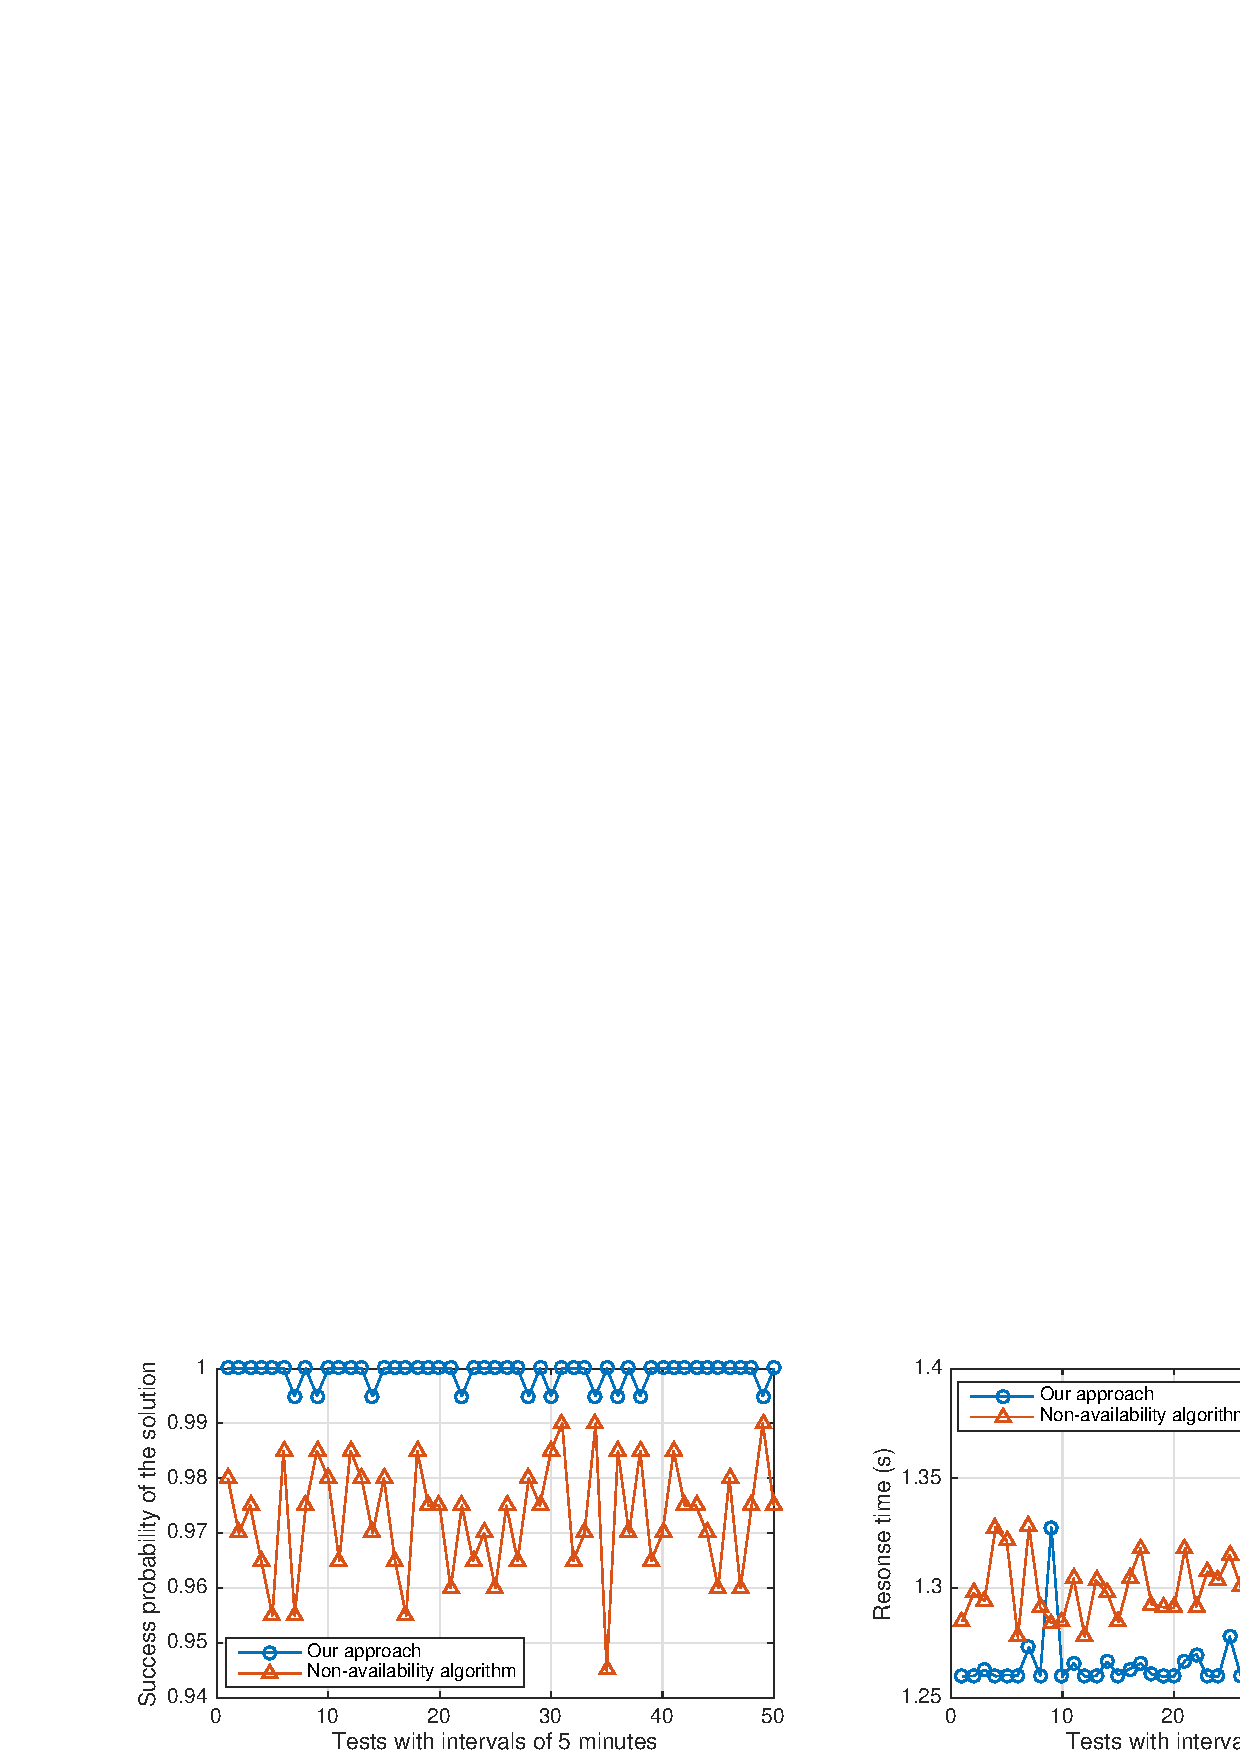
\includegraphics[width=6.6in]{./img/Task-6.pdf}
\caption{Case study for travel arrange}
\label{Task-6}
\end{figure*}
\begin{figure*}[!t]
\centering
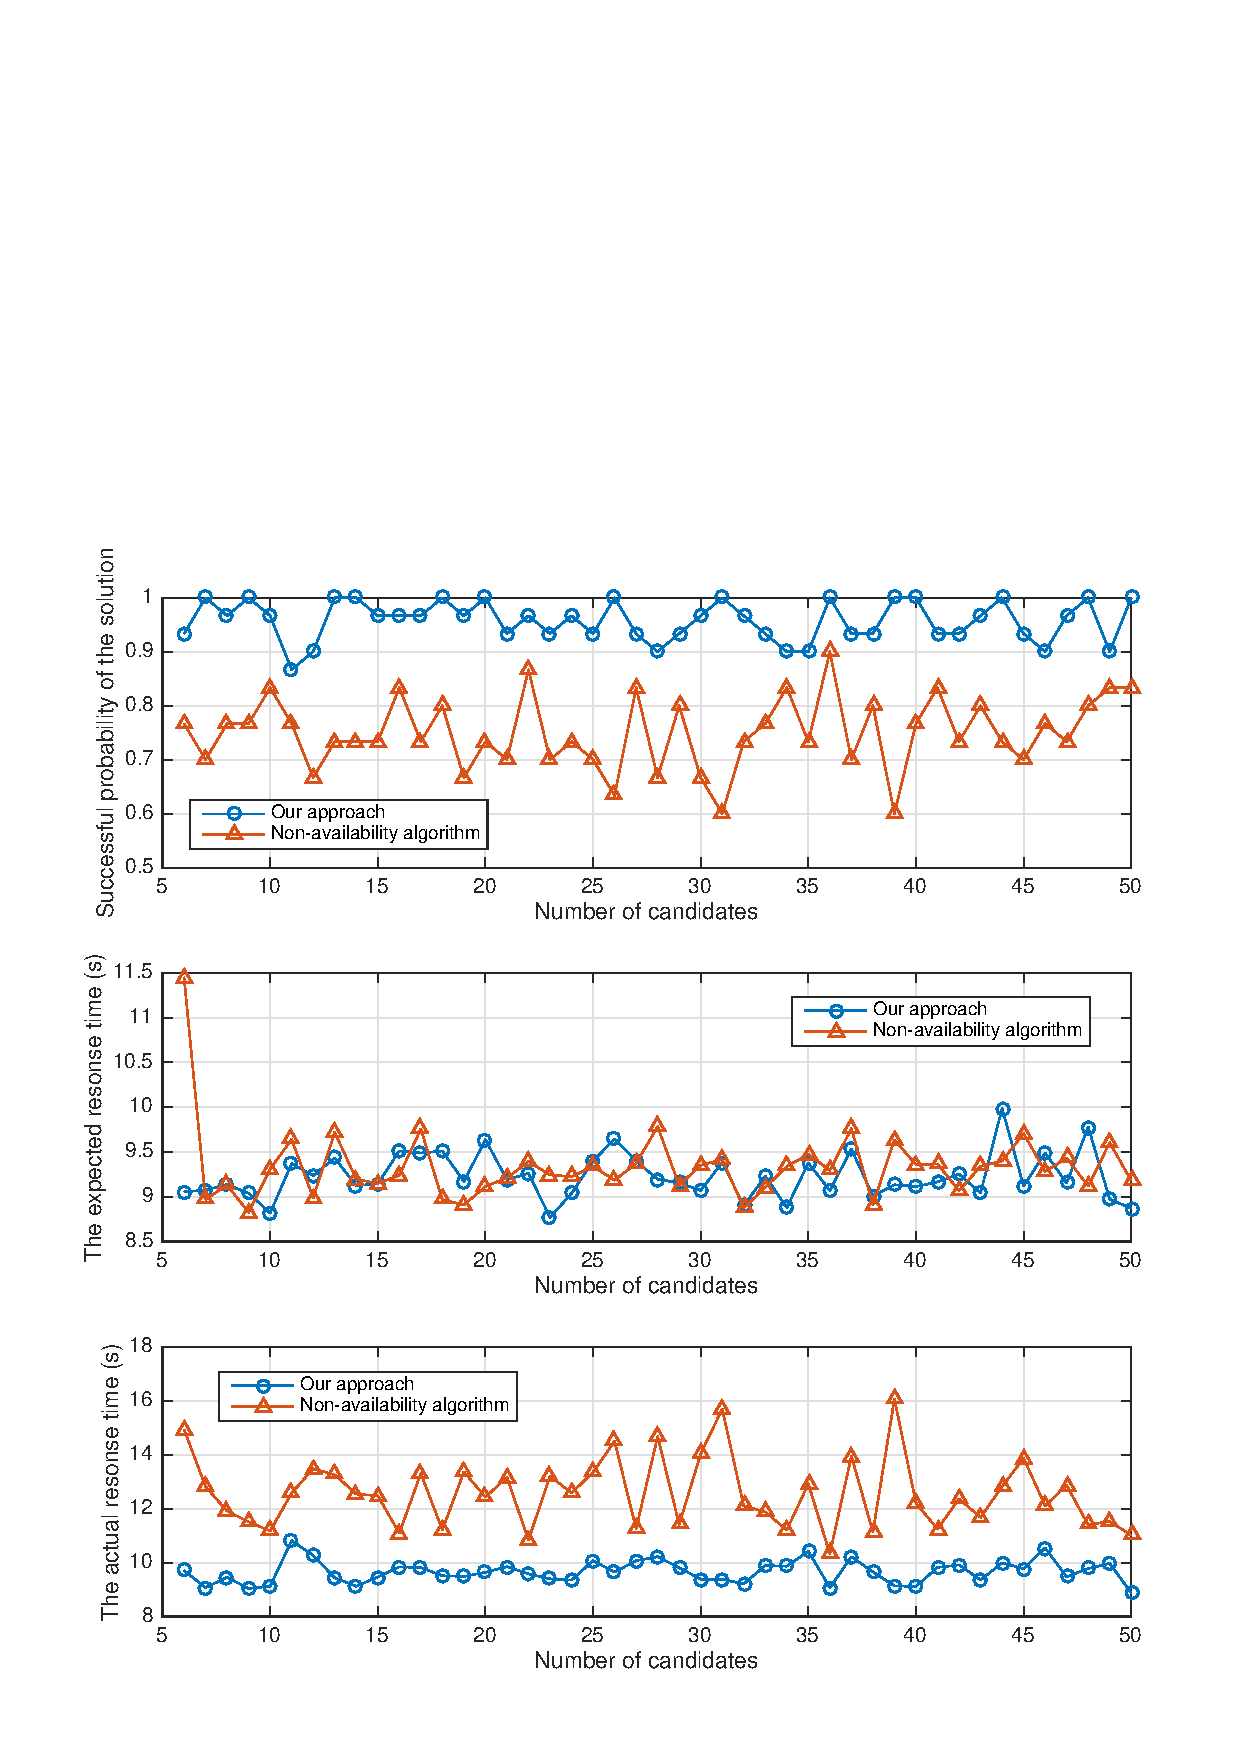
\includegraphics[width=6.6in]{./img/Task-12.pdf}
\caption{Case study for tensorflow}
\label{Task-12}
\end{figure*}
\begin{figure*}[!t]
\centering
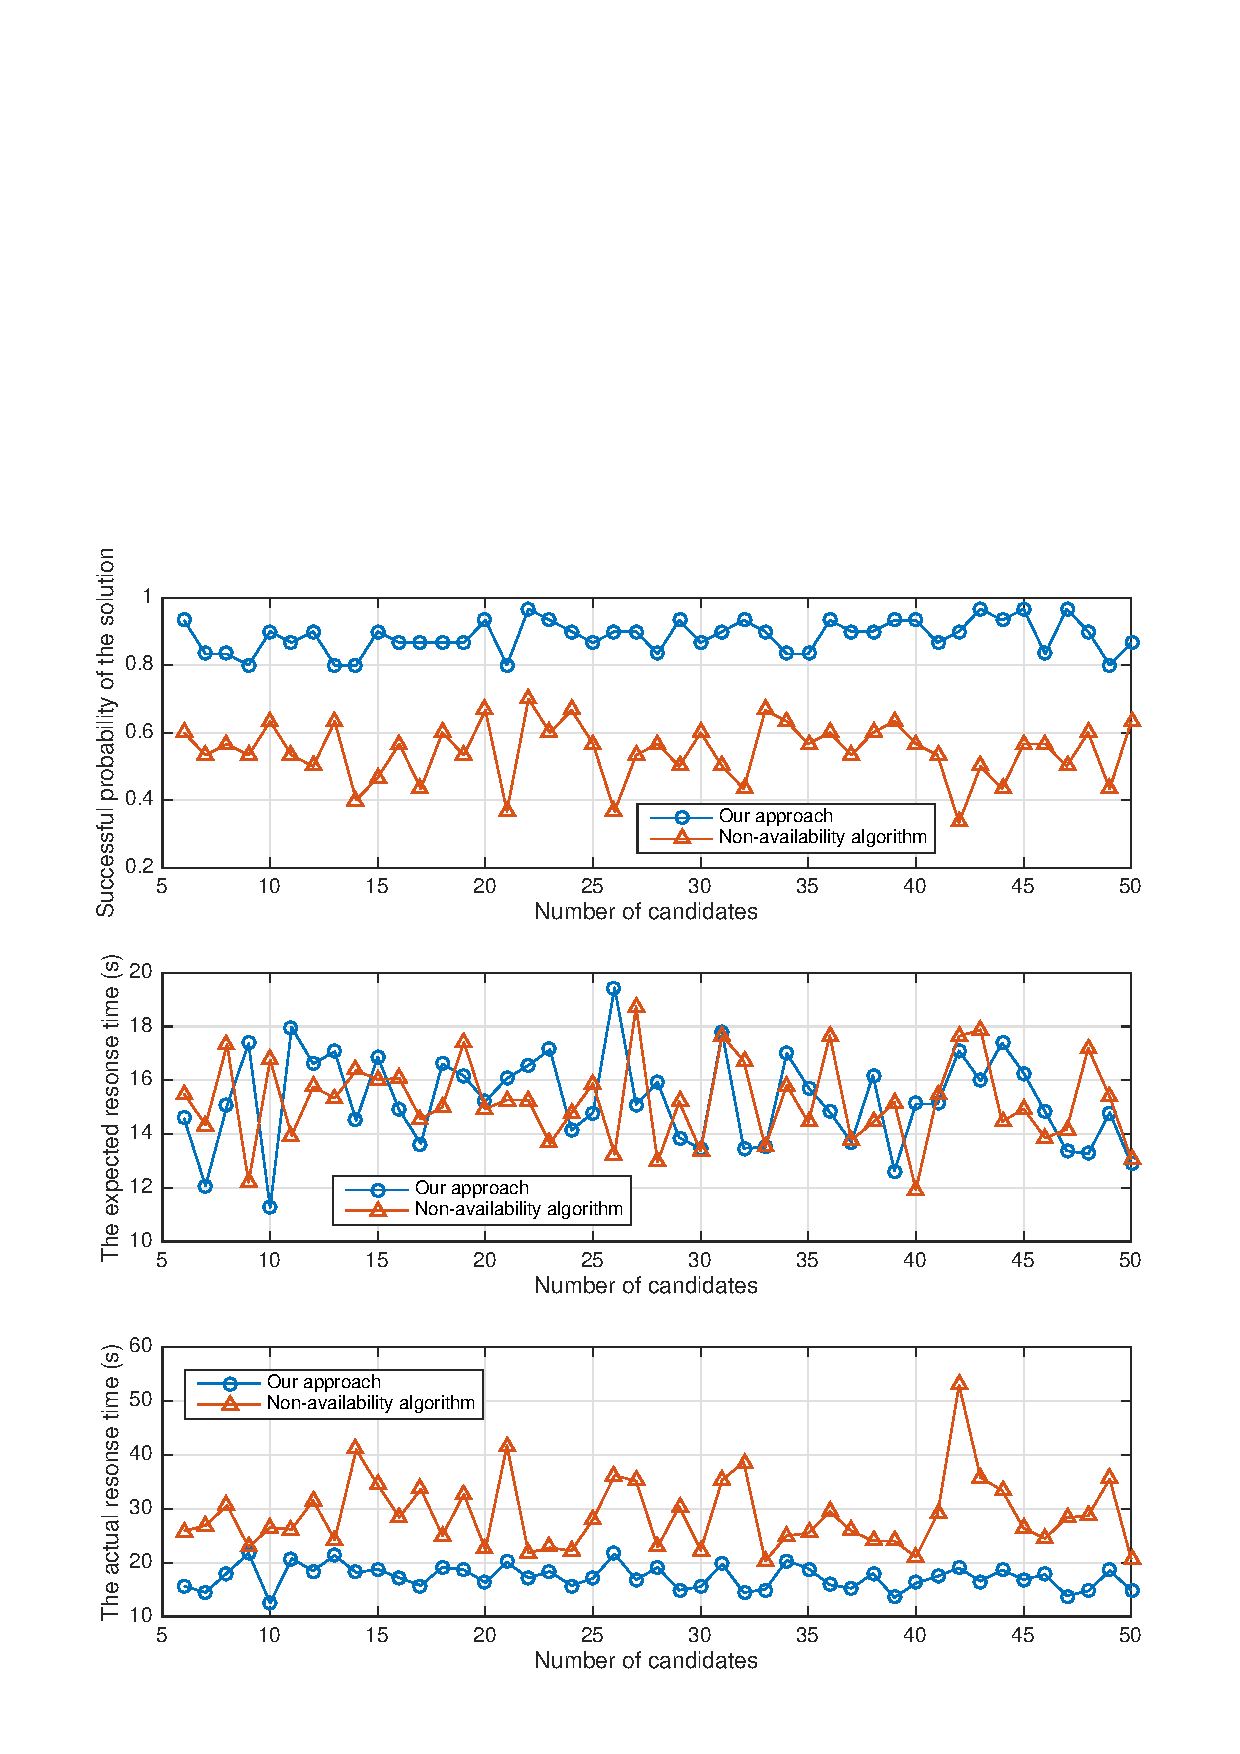
\includegraphics[width=6.6in]{./img/Task-24.pdf}
\caption{Case study for montage}
\label{Task-24}
\end{figure*}
\begin{figure*}[!t]
\centering
\includegraphics[width=6.6in]{./img/Task-12-random.pdf}
\caption{Case study for random generated composition template}
\label{Task-random}
\end{figure*}

As shown in Fig. 9(a), Fig. 10(a), Fig. 11(a) and Fig. 12(a), our proposed method achieves higher success rate ($99.9\%$ vs. $97.3\%$ for Case I in average, $92.1\%$ vs. $75.7\%$ for Case II in average, and $89\%$ vs. $54.9\%$ for Case III in average, and $91.8\%$ vs. $75.6\%$ for Case IV in average) compared with its peers.
Fig. 9(b), Fig. 10(b), Fig. 11(b) and Fig. 12(b) shows the comparisons of process completion time where our proposed algorithm achieves 2.2\%, 17.7\%, 38.2\%, and 18.8\% time savings in each case over its peer. 
Intuitively, our algorithm outperforms traditional ones because traditional ones consider fully available mobile services and thus they tend to choose services with low response time. As a result, the service composition constructed by these low response time services might have a poor reliability and would eventually lead to a failure.

\section{Conclusion}
This paper presents a comprehensive framework for optimal mobile service composition in a mobile environment. It fully leverages service mobility with a reliability-aware and deadline-constrained mobile service composition model. Then we formulate the developed model as an optimization problem aiming at maximizing the quality of composite service and propose a Krill-Herd-based algorithm to solve it. We also carry out a case study based on a real-world opportunistic network and some well-known mobile service composition templates and shows that our proposed approach outperforms traditional non-reliability approaches, especially those who consider constant/time-invariant availability of mobile services, in terms of success rate and completion time.

The following issues should be addressed as future work: 1) Some prediction methods, e.g., time-series model, hidden Markov models and neural networks can be used to predict a user's future movement and to achieve further improved performance of composite services; 2) more metrics, e.g., service scalability and service reputation should be modeled and  analyzed; 3) soft constraints should be considered. They allow to exceed a threshold value with a bounded given rate, while the corresponding algorithms for optimal run-time scheduling should be developed.



% Can use something like this to put references on a page
% by themselves when using endfloat and the captionsoff option.
\ifCLASSOPTIONcaptionsoff
  \newpage
\fi




\bibliography{mybibtex}
\bibliographystyle{IEEEtran}
\end{document}


